\begin{figure}
  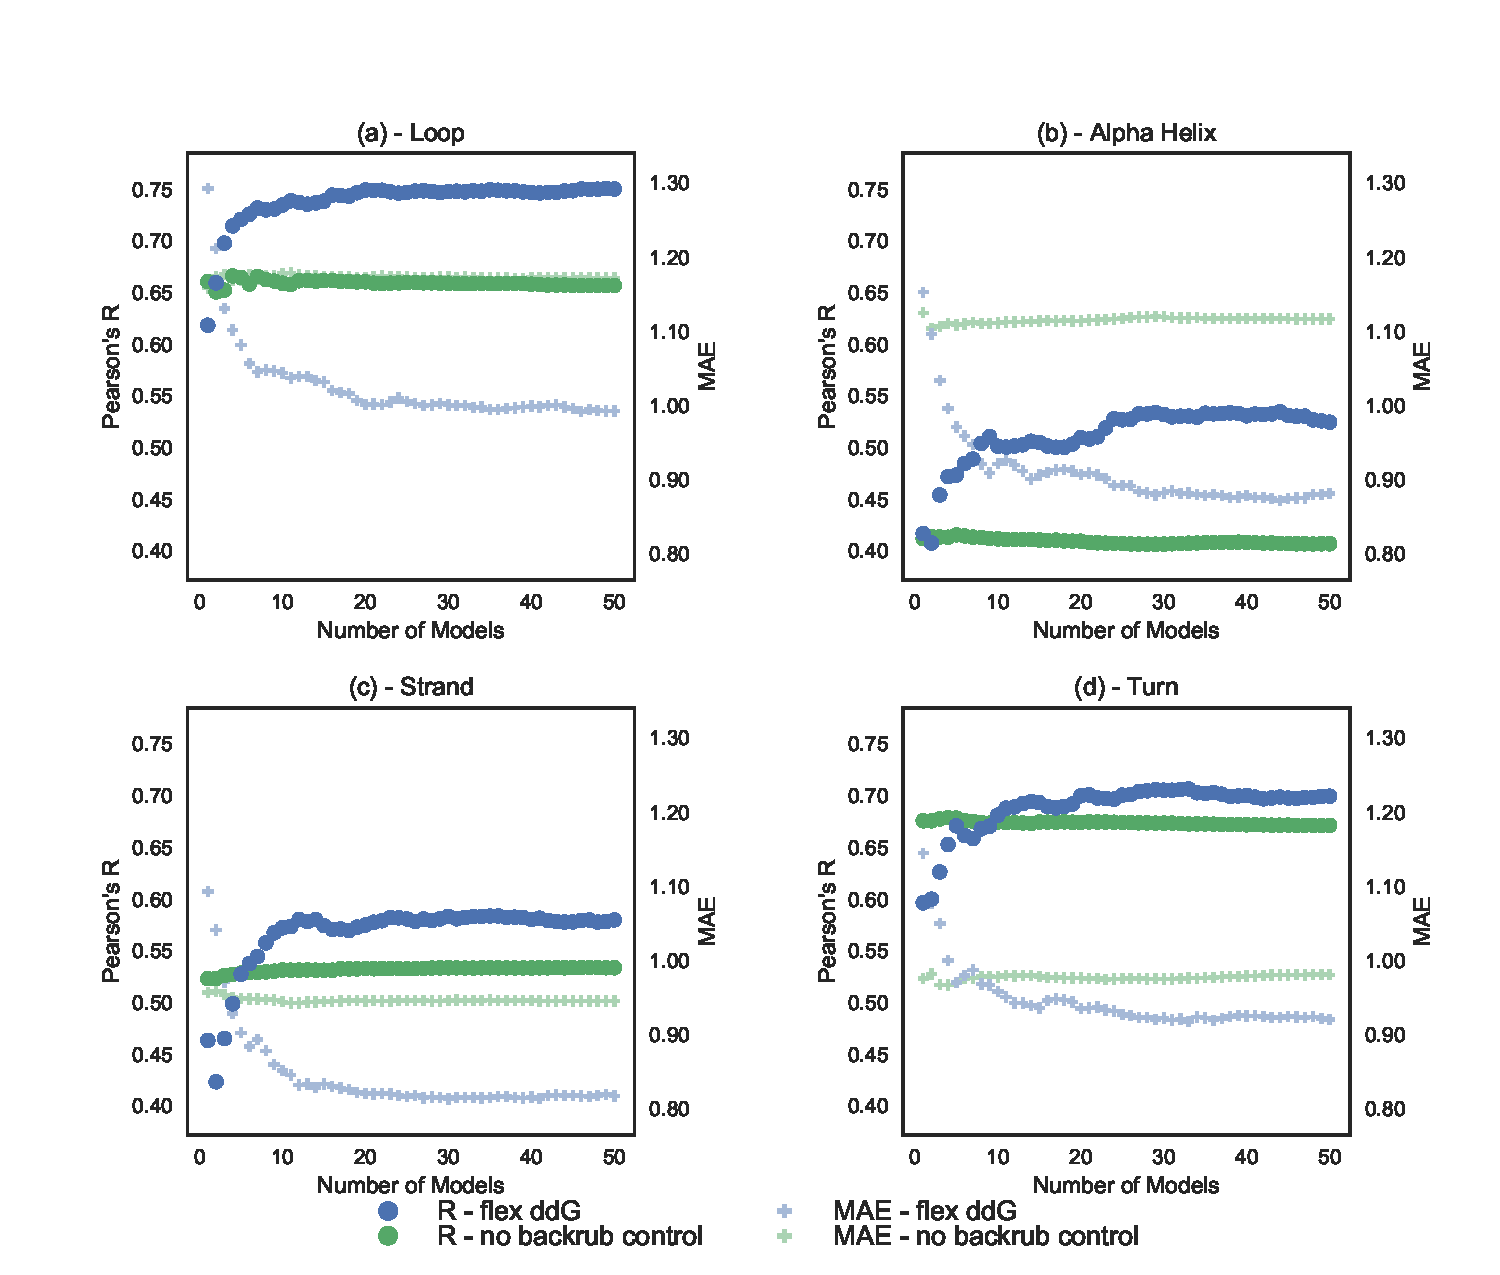
\includegraphics[width=\textwidth,keepaspectratio]{structs-v-corr-id-zemu-12-60000-rscript-simplified-t14-SS.pdf}
  \caption[]{
    Correlation (Pearson's R, left y-axis) and MAE (Mean Absolute Error, right y-axis) vs. number of averaged models (x-axis), on subsets of the complete ZEMu set binned by DSSP-assigned\cite{kabsch_dictionary_1983,joosten_series_2011}\ secondary structure at the mutation site. For cases with multiple mutations, all mutation sites must share the same secondary structure to be considered.
    Pearson's R is shown as circles, and MAE as faded plusses.
Predictions generated with the Flex ddG protocol are shown in blue.
Predictions generated with the no backrub control protocol are shown in green.
    A selection of key data underlying this figure can be found in \cref{tab:structs-v-corr-id-zemu-12-60000-rscript-simplified-t14-SS-underlying-data}. Flex ddG is run with 35000 backrub steps.
    Structures are not sorted, and are randomly added to the ensemble.
    (a) Loop (n = 349)
    (b) Alpha helix (n = 198)
    (c) Strand (n = 280)
    (d) Turn (n = 183).
  } \label{fig:structs-v-corr-id-zemu-12-60000-rscript-simplified-t14-SS}
\end{figure}
